\documentclass[11pt,aspectratio=169]{beamer}

%% ==== Theme ==============================================================
\usetheme{Madrid}
\usecolortheme{whale}
\setbeamertemplate{navigation symbols}{}
\setbeamertemplate{footline}[frame number]
\setbeamercovered{transparent}

%% ==== Packages ============================================================
\usepackage[T1]{fontenc}
\usepackage{lmodern}
\usepackage{amsmath,amssymb}
\usepackage{booktabs}
\usepackage{tikz}
\usetikzlibrary{arrows.meta,positioning}

\title[Familiarity \& Peer Effects]{Does Repeated Exposure to Peers\\Change the Peer Effect?}
\subtitle{Learning, Incentives, and Rivalry Among Competitive Runners}
\author{Mahyar Rezazadeh}
\institute{Meeting with Fernando}
\date{\today}

\begin{document}

%% ---------------------------------------------------------------------
\begin{frame}
\titlepage
\end{frame}

%% ---------------------------------------------------------------------
\begin{frame}{Roadmap}
\begin{enumerate}
    \item State of the problem
    \item Why this question matters
    \item Research question \& candidate mechanisms
    \item Setting and data (brief)
    \item Questions for discussion
\end{enumerate}
\end{frame}

%% ---------------------------------------------------------------------
\begin{frame}{Motivating Observation}
\begin{itemize}
    \item Magic Johnson read Larry Bird's box scores every morning.
    \item Federer's game reportedly changed whenever Nadal was across the net.
    \item Radcliffe credited Gete Wami's presence for pushing her to a
          world-record pace in the 2003 London Marathon.
\end{itemize}
\vspace{0.5em}
\begin{block}{Common thread}
It is not just \emph{how good} the field is --- it is \emph{who} you have
faced before, and how many times.
\end{block}
\end{frame}

%% ---------------------------------------------------------------------
\begin{frame}{State of the Problem}
\small
\begin{itemize}
    \item Peer-effects models treat every opponent as
          \textbf{interchangeable}: what matters is the average (or max/min)
          quality of the field, not the identity or history of any one rival.
    \begin{itemize}
        \item Linear-in-means and the eight HOX (2007) mechanisms all take a
              \emph{static} peer statistic as the input.
        \item Boucher (2024) generalizes the response function, but the
              peer group's relationship history still plays no role.
    \end{itemize}
    \item Separately, sports psychology (Kilduff et al., 2010, 2014)
          documents that \textbf{rivals} --- opponents defined partly by
          repeated encounters --- are psychologically distinct from
          generic competitors.
    \item These two literatures have not been connected: no large-scale
          study asks whether the \emph{same} opponent quality produces a
          \emph{different} peer effect depending on how many times the pair
          has already competed.
\end{itemize}
\vspace{0.3em}
\begin{alertblock}{The gap}
We do not know whether the peer effect is a fixed parameter, or whether it
evolves with the history of interaction between competitors.
\end{alertblock}
\end{frame}

%% ---------------------------------------------------------------------
\begin{frame}{Why This Question Matters}
\begin{columns}[T]
\begin{column}{0.5\textwidth}
\textbf{Theoretical}
\begin{itemize}
    \item If the peer-effect coefficient depends on relational history,
          estimates that pool first encounters with long-standing rivalries
          are averaging over two different regimes.
    \item Distinguishing \emph{learning} from \emph{incentive/rivalry}
          channels has different comparative statics and different
          predicted dynamics.
\end{itemize}
\end{column}
\begin{column}{0.5\textwidth}
\textbf{Practical}
\begin{itemize}
    \item Repeated competitive matchups are everywhere: sales contests,
          grant competitions, promotion tournaments, school tracking,
          recurring sports fixtures.
    \item Individual-sport running \textbf{isolates} rivalry-driven peer
          effects from the altruism confound that plagues team-sport
          estimates --- a clean setting for a general organizational
          question.
\end{itemize}
\end{column}
\end{columns}
\end{frame}

%% ---------------------------------------------------------------------
\begin{frame}{Research Question}
\begin{block}{}
\centering
\Large How does the effect of an opponent's quality on a focal athlete's
performance change with the number of times the two have previously
competed against each other?
\end{block}
\vspace{1em}
\textit{Familiarity:} $f_{ij,t} = \#\{\text{prior races of } i \text{ against } j
\text{ before } t\}$.
\end{frame}

%% ---------------------------------------------------------------------
\begin{frame}{Two Candidate Mechanisms}
\small
\begin{columns}[T]
\begin{column}{0.48\textwidth}
\begin{block}{Learning / information}
A first encounter reveals a lot about an unfamiliar opponent's current form.
As uncertainty resolves, the informational value of the peer signal --- and
the peer effect --- should \textbf{shrink} with repetition.
\end{block}
\end{column}
\begin{column}{0.48\textwidth}
\begin{block}{Incentives / rivalry}
Repeated matchups raise the psychological and reputational stakes of a
head-to-head. As familiarity builds, the incentive to outperform a known
rival should \textbf{grow} with repetition.
\end{block}
\end{column}
\end{columns}

\vspace{0.5em}
\begin{center}
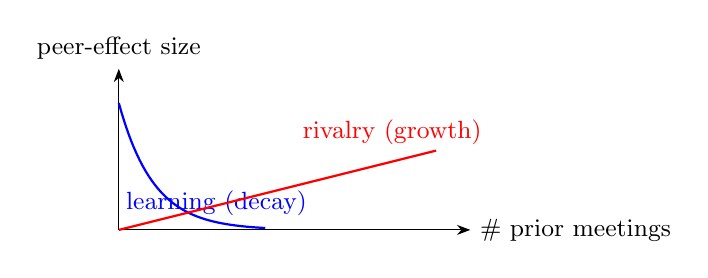
\begin{tikzpicture}[scale=0.62]
\draw[-Stealth] (0,0) -- (7.2,0) node[right] {\small \# prior meetings};
\draw[-Stealth] (0,0) -- (0,3.3) node[above] {\small peer-effect size};
\draw[thick,blue,domain=0:3,samples=50] plot (\x,{2.6*exp(-1.4*\x)}) ;
\node[blue] at (2.0,0.55) {\small learning (decay)};
\draw[thick,red,domain=0:6.5,samples=50] plot (\x,{0.25*\x});
\node[red] at (5.6,2.0) {\small rivalry (growth)};
\end{tikzpicture}

\small Both channels together can generate a non-monotonic (e.g.\ U-shaped)
profile --- an empirical question, not an assumption.
\end{center}
\end{frame}

%% ---------------------------------------------------------------------
\begin{frame}{Identifying the Mechanisms with Current Data}
\scriptsize
No experiment separates them cleanly --- the strategy is a set of
\textbf{differential predictions}, all computable from variables already on
file (race dates, round/tier, age, nationality). A convergent pattern across
tests is what would be persuasive, not any single one.

\vspace{0.3em}
\begin{tabular}{@{}p{2.6cm}p{3.5cm}p{3.5cm}@{}}
\toprule
\textbf{Test} & \textbf{Learning predicts} & \textbf{Rivalry predicts} \\
\midrule
\textbf{Recency}: time since last co-race vs.\ raw meeting count &
Effect fades as elapsed time grows (stale information) &
Effect persists regardless of elapsed time \\[0.35em]
\textbf{Precision}: variance of residual performance by familiarity bin &
Residual variance shrinks (uncertainty resolved) &
Variance flat; only the mean response shifts \\[0.35em]
\textbf{Stakes}: familiarity $\times$ final / championship round &
Amplification stakes-invariant &
Amplification concentrated in high-stakes rounds \\[0.35em]
\textbf{Experience}: familiarity $\times$ athlete's career race count &
First-meeting drop largest for novices &
High-familiarity amplification flat across experience \\
\bottomrule
\end{tabular}

\vspace{0.3em}
\textit{Robustness:} re-run each test instrumenting familiarity with
geographic distance between athletes' nationalities (already used for the
endogeneity check) to rule out selection into repeat matchups as the driver.
\end{frame}

%% ---------------------------------------------------------------------
\begin{frame}{Setting and Data (brief)}
\begin{itemize}
    \item World Athletics Organization competition records, 2005--2023:
          $\sim$587{,}000 race observations, $\sim$49{,}000 athletes,
          $\sim$5{,}180 competitions, 1{,}500+ cities.
    \item Individual track events: no team production $\Rightarrow$
          rules out the altruism confound present in team-sport peer-effect
          studies.
    \item Full opponent history per athlete lets us construct familiarity
          $f_{ij,t}$ from actual head-to-head competition records, not a
          proxy.
    \item Opponent quality is built from \emph{prior} (predetermined)
          performance only, sidestepping the reflection problem
          (Manski, 1993).
\end{itemize}
\end{frame}

%% ---------------------------------------------------------------------
\begin{frame}{Questions for Discussion}
\begin{itemize}
    \item Which mechanism story is most convincing \emph{ex ante} --- and
          is there a third channel we are missing?
    \item How do we cleanly separate learning from incentive effects
          empirically, rather than just describing the reduced-form shape?
    \item What is the sharpest falsification test for each mechanism?
    \item Does the framing of the question (state of the problem \&
          motivation) hold up, before we go further into identification
          and estimation?
\end{itemize}
\end{frame}

\end{document}
